% Where the shipped model's error sits in frequency and in space, and the
% Delta-alpha gated spectral-profile loss that follows from it. Running log: sections
% are appended as each step lands. TODO.md section 44 points here.
% Compile from inside reports/:  ~/anaconda3/envs/tex/bin/tectonic error_spectrum_report.tex
\documentclass[10pt,a4paper]{article}

\usepackage[margin=18mm]{geometry}
\usepackage{booktabs}
\usepackage{xcolor}
\usepackage{graphicx}
\usepackage{caption}
\usepackage{float}
\usepackage{amsmath}
\usepackage{amssymb}
\usepackage{enumitem}
\usepackage[colorlinks=true,linkcolor=black,urlcolor=black]{hyperref}

\definecolor{accent}{HTML}{D64545}
\definecolor{cond}{HTML}{3E7CB1}
\definecolor{ink}{HTML}{102A43}
\definecolor{muted}{HTML}{627D98}
\definecolor{live}{HTML}{D9822B}

\captionsetup[figure]{font=small,labelfont=bf}
\captionsetup[table]{font=small,labelfont=bf}
\setlist[itemize]{itemsep=0.6mm,topsep=1mm}
\setlength{\parindent}{0pt}
\setlength{\parskip}{1.2mm}

% a number or a result not measured yet; grep for \pending before calling a section done
\newcommand{\pending}[1][pending]{\textcolor{live}{\textit{#1}}}
\newcommand{\da}{\Delta\alpha}

\begin{document}
\sloppy

{\Large\bfseries Error spectrum and the $\Delta\alpha$-gated spectral loss}\\[1mm]
{\small Task 3 running log. Section numbers in brackets are \texttt{TODO.md}.
Status: post-hoc detail gain negative, SSIM weight above 0.5 not run (\S\ref{sec:next});
spectral loss dropped on analysis (\S\ref{sec:loss}), then trained: $-0.00118$ local SSIM,
challenge \pending[not submitted] (\S\ref{sec:losstest}).}

% ======================================================================
\section{Starting point}\label{sec:start}

\begin{itemize}
  \item Shipped model: \texttt{task3\_mc\_ssim\_slice}, mean of e6/e7/e8 weights, 4-flip TTA.
        Challenge \textbf{SSIM 0.913652}, nRMSE 0.237970, LPIPS 0.090899 [\S40].
  \item 32-channel conditional U-Net, 4-channel multi-contrast input, MIM pretrained on 1{,}939
        unpaired volumes, conditioned on $c = E_{\mathrm{src}} + E_{\mathrm{tgt}} + E_z$.
  \item Error by field [\S30, \texttt{error\_by\_field.pdf}]: 0.1\,T is 40\% of the
        transitions and 50\% of $\sum(1-\mathrm{SSIM})$.
  \item Spectral slopes [\texttt{spectral/alpha\_summary.csv}, retrospective split]:
        0.1\,T sits $\da = +1.01$ to $+1.50$ steeper than 7\,T, so it carries almost none of
        7\,T's high-frequency power; 3\,T and 5\,T are within $\pm 0.5$.
  \item Qualitative [\texttt{figures/slide\_two\_regimes.pdf}]: at 0.1\,T the residual sits on
        the cortical folds; at 3\,T only on the outer brain edge.
\end{itemize}

% ======================================================================
\section{What is already closed}\label{sec:closed}

Ideas that read as next steps but were measured. A local delta under 0.001 is not evidence
[\S32]; a 0009-only margin needs about 0.0025.

\begin{table}[H]
\centering\small
\begin{tabular}{llr}
\toprule
Idea & Section & Result \\
\midrule
0.1\,T loss weight 0.5                & \S31   & $-0.0017$ local \\
3-model ensemble                      & \S20   & $+0.0011$ local \\
2.5D input ($z\pm2$)                  & \S34   & 0.909353 \\
axial token on top of 2.5D            & \S39   & $-0.0010$ local \\
more MIM pretraining (60k steps)      & \S21.1 & $+0.0007$ local \\
SSIM loss weight 0.10 / 0.25          & \S28.6 & 0.5 wins \\
FiLM \& residual head                 & \S9    & 0.892839 \\
50/50 soup with a sibling run         & \S40   & 0.913203 \\
conditional flow matching, 3 stages   & \S38   & 0.886725 \\
\bottomrule
\end{tabular}
\caption{Closed lines. Scores are challenge SSIM unless marked local.}
\end{table}

Still open before this report:
\begin{itemize}
  \item \texttt{avg\_e4\_e8} + TTA: built, never submitted [\S40].
  \item 2.5D + averaging + TTA: never tried.
  \item B5, spectral-profile loss: proposed, never implemented [\S2].
\end{itemize}

% ======================================================================
\section{Plan and the reasoning behind it}\label{sec:plan}

Hypothesis: most of the remaining error sits on non-smooth, high-frequency structure (outer brain
edge, cortical folds) at \emph{every} field, not only at 0.1\,T.

Three ways to use $\da$, and why two were rejected:
\begin{itemize}
  \item \textbf{$\da$ as a conditioning input. Rejected.} $\da$ is a fixed lookup of
        (modality, source, target), the triple the embeddings already see. No new information;
        all 60 cells are in training, so its ordering prior has nothing to generalise to.
        Same profile as the axial token ($+0.0006$).
  \item \textbf{$|\da|$ as a per-pair loss weight. Rejected.} $|\da|$ is 0.85 to 1.72 on every
        0.1\,T cell and at most 0.66 elsewhere, so it reproduces \S31's 0.1\,T weighting
        ($-0.0017$), and the absolute value drops the direction that \S31 showed matters.
  \item \textbf{$\da$ gating a spectral-profile loss. Kept.} The loss acts only when the target
        is smoother than the source, where matching its spectrum means \emph{removing} detail.
        That agrees with SSIM. In the other direction the detail is not in the input, and
        matching power means inventing texture, the LPIPS-for-SSIM trade [\S28.1, \S40].
\end{itemize}

Sign convention used from here on (the slides use the opposite one):
\[
  \da_{s\to t} = \alpha_t - \alpha_s, \qquad
  \da_{s\to t} > 0 \iff \text{target smoother than source (away from high field)}.
\]

Order of work, each step gating the next:
\begin{enumerate}[itemsep=0.6mm,topsep=1mm]
  \item Error spectrum and edge analysis of the shipped model (\S\ref{sec:analysis}). Stop if the
        error is not concentrated in the mid/high band or on edges.
  \item Implement the gated loss (\S\ref{sec:loss}).
  \item Ablate A0 to A3 locally; submit only arms that clear $+0.001$ (\S\ref{sec:loss}).
        Budget: 5 submissions per day.
\end{enumerate}

% ======================================================================
\section{Error spectrum and edge analysis}\label{sec:analysis}

\textbf{Setup}
\begin{itemize}
  \item Script: \texttt{scripts/error\_spectrum\_analysis.py}. Inference through
        \texttt{make\_task3\_submission}\allowbreak\texttt{.predict\_slab}, the path that produced the upload.
  \item Weights \texttt{docker/task3/weights/task3.pt}, 4-flip TTA. 3 subjects (0006, 0007,
        0009) $\times$ 3 modalities $\times$ 20 transitions $=$ 180, submission slab $z \in
        [150, 180)$.
  \item Error $e = \hat y\cdot\mathbb{1}[x > 10^{-3}] - y$, the challenge's masking.
  \item Caveat: every config has \texttt{holdout\_subjects = []}, so all three subjects were in
        training. Absolute errors are optimistic; how the error \emph{splits} is what is read.
\end{itemize}

\textbf{Frequency}
\begin{itemize}
  \item RAPSD of $e$, of $y$, and of the copy baseline's error $x - y$, per slice,
        zero-padded to square (not cropped: a crop cuts through the head and leaks a hard edge
        into every bin).
  \item Bands in cycles/pixel: low $< 0.05$, mid $0.05$--$0.20$, high $> 0.20$.
        Mid matches the $\alpha$ fit band.
\end{itemize}

\textbf{Space}
\begin{itemize}
  \item Per-pixel error: $1 - \mathrm{SSIM}$ map (the ranked metric) and $e^2$.
  \item Edge strength $|\nabla y|$ (Sobel on the target), binned into deciles inside the brain.
  \item Three regions: \emph{outer edge} (within 4\,px of the brain boundary), \emph{folds}
        (interior, top 20\% of $|\nabla y|$), \emph{flat} (the rest). Enrichment
        $=$ error share / pixel share.
\end{itemize}

\textbf{Results.} 168 transitions (the 12 T2W$\to$1.5\,T cells are excluded: corrupt
ground truth). Local SSIM 0.9526, copy baseline 0.8343.
Data: \texttt{error\_spectrum/summary.csv}, \texttt{per\_transition.csv}, \texttt{spectra.npz}.

\begin{figure}[H]
\centering
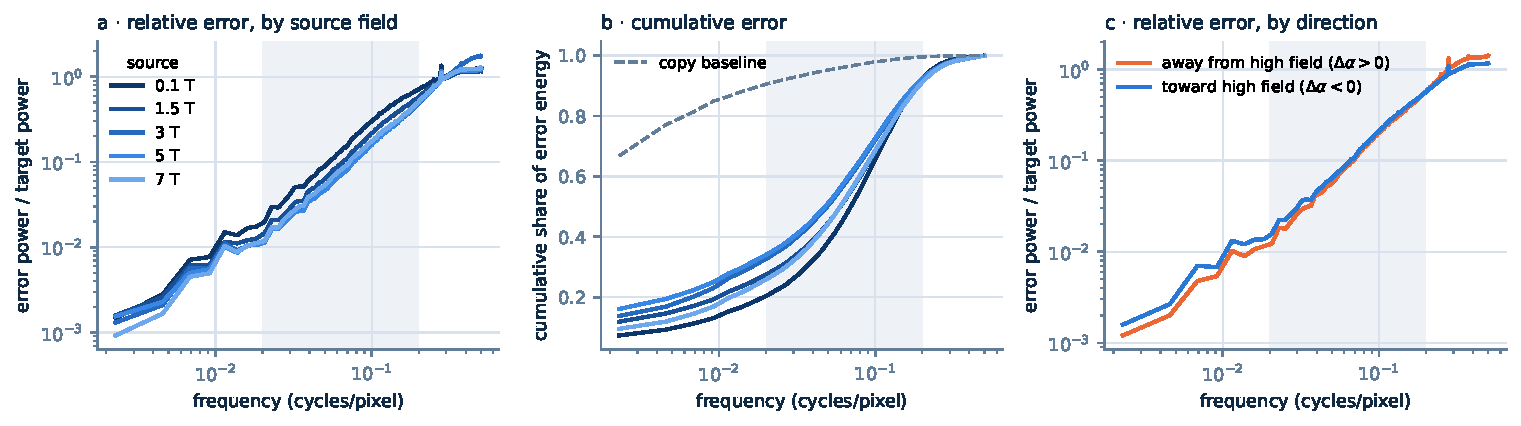
\includegraphics[width=\textwidth]{spectral/fig_error_rapsd_by_field.pdf}
\caption{Error spectrum. Shaded: the $\alpha$ fit band, 0.02--0.20 cycles/pixel.}
\label{fig:rapsd}
\end{figure}

\begin{table}[H]
\centering\small
\begin{tabular}{lllrrrrr}
\toprule
Panel & Quantity & Group & $<0.05$ & $0.05$--$0.1$ & $0.1$--$0.2$ & $0.2$--$0.3$ & $>0.3$ \\
\midrule
\ref{fig:rapsd}.a & $P_e / P_y$ & all            & 0.029 & 0.107 & 0.322 & 0.724 & 1.153 \\
\ref{fig:rapsd}.a & $P_e / P_y$ & source 0.1\,T  & 0.044 & 0.159 & 0.452 & 0.841 & 1.147 \\
\ref{fig:rapsd}.c & $P_e / P_y$ & $\da>0$ (away)   & 0.027 & 0.102 & 0.307 & 0.756 & 1.283 \\
\ref{fig:rapsd}.c & $P_e / P_y$ & $\da<0$ (toward) & 0.033 & 0.112 & 0.332 & 0.710 & 1.069 \\
\ref{fig:rapsd}.b & $P_e / P_{x-y}$ & all        & 0.10  & 0.26  & 0.42  & 0.54  & 0.61 \\
\bottomrule
\end{tabular}
\caption{Error power relative to the target (rows 1--4) and to the copy baseline's error
(row 5), per frequency band in cycles/pixel. The $<0.05$ column covers 0.02--0.05 only.}
\label{tab:bands}
\end{table}

\begin{itemize}
  \item \textbf{The model has solved the low frequencies.} Below 0.02 cycles/pixel the error is
        1\% of the copy baseline's; the baseline's error is 96.7\% low band, the model's 47.4\%
        low, 45.0\% mid, 7.6\% high (Figure~\ref{fig:rapsd}.b).
  \item \textbf{Relative error rises monotonically with frequency} at every source field:
        3\% of target power at 0.02--0.05, 32\% at 0.1--0.2, and \emph{above} the target's own
        power past 0.3 (Table~\ref{tab:bands}). Above $\sim$0.3 cycles/pixel the prediction is
        uncorrelated with the target.
  \item \textbf{Direction does not separate the spectra.} Away and toward curves overlap within
        10\% in every band (Figure~\ref{fig:rapsd}.c). The $\da$ gate selects transitions,
        not a spectral deficit.
  \item 0.1\,T as source sits 1.4--1.5$\times$ higher in the low and mid bands, the only field
        that separates (Figure~\ref{fig:rapsd}.a).
  \item A narrow spike near 0.29 cycles/pixel ($\approx$3.4\,px period) appears in every group;
        not investigated.
\end{itemize}

\begin{figure}[H]
\centering
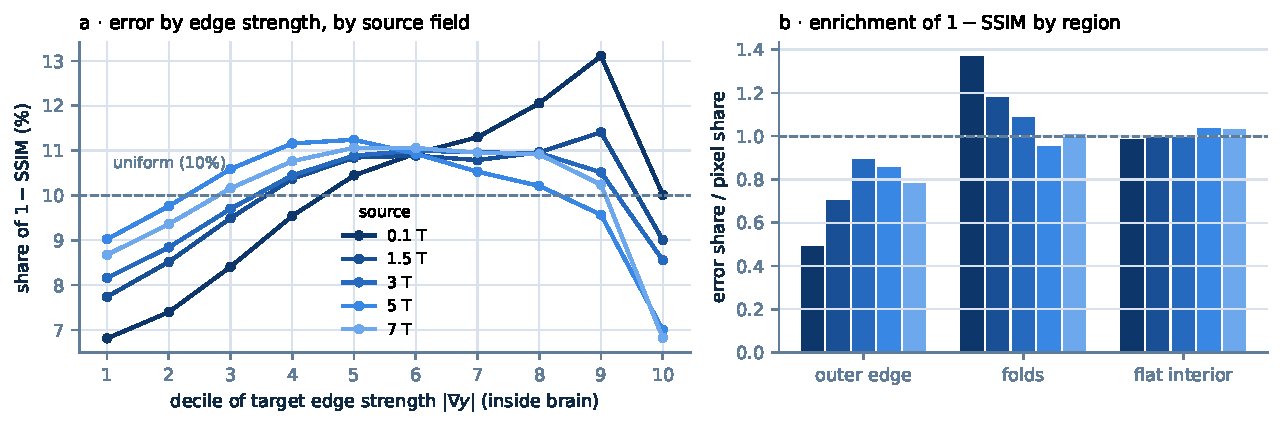
\includegraphics[width=0.92\textwidth]{spectral/fig_error_by_edge.pdf}
\caption{Spatial split of the ranked metric's deficit. Colours as in Figure~\ref{fig:rapsd}.a.}
\label{fig:edge}
\end{figure}

\begin{table}[H]
\centering\small
\begin{tabular}{llrrrrrr}
\toprule
Panel & Source & \multicolumn{3}{c}{$1-\mathrm{SSIM}$ enrichment} & top-2 deciles
      & $e^2$ folds & $\rho(|e|, |\nabla y|)$ \\
\cmidrule(lr){3-5}
 & & edge & folds & flat & of $1-\mathrm{SSIM}$ & enrichment & \\
\midrule
\ref{fig:edge}.b & all    & 0.71 & 1.14 & 1.00 & 19.7\% & 1.97 & 0.19 \\
\ref{fig:edge}.b & 0.1\,T & 0.49 & 1.36 & 0.98 & 23.1\% & 2.34 & 0.27 \\
\ref{fig:edge}.b & 1.5\,T & 0.69 & 1.17 & 0.99 & 20.4\% & 2.09 & 0.19 \\
\ref{fig:edge}.b & 3\,T   & 0.90 & 1.08 & 0.98 & 19.1\% & 1.73 & 0.17 \\
\ref{fig:edge}.b & 5\,T   & 0.85 & 0.94 & 1.03 & 16.6\% & 1.64 & 0.14 \\
\ref{fig:edge}.b & 7\,T   & 0.77 & 1.00 & 1.02 & 17.1\% & 1.79 & 0.20 \\
\bottomrule
\end{tabular}
\caption{Enrichment $=$ error share / pixel share (pixels: edge 10.3\%, folds 17.9\%, flat
71.7\%). Top-2 deciles: share of $1-\mathrm{SSIM}$ in the 20\% strongest-edge pixels.}
\label{tab:edge}
\end{table}

\begin{itemize}
  \item \textbf{Squared error does follow the edges, at every field.} Folds hold 35.3\% of $e^2$
        on 17.9\% of the pixels: 1.6--2.3$\times$ enrichment, 0.1\,T highest, 5\,T lowest.
        This is what the residual maps showed.
  \item \textbf{The ranked metric does not.} $1-\mathrm{SSIM}$ is spread like the pixels:
        19.7\% in the top-2 edge deciles against 20\% uniform, flat interior 1.00, outer edge
        under-weighted at 0.71 (Table~\ref{tab:edge}).
  \item Why: SSIM divides by local variance, so an error on a high-contrast fold costs less than
        the same error on flat tissue. 72\% of the deficit is in the flat interior, which is
        72\% of the area.
  \item Only 0.1\,T and 1.5\,T as source put extra $1-\mathrm{SSIM}$ on folds (1.36, 1.17),
        and the deciles peak at decile 9, not 10 (Figure~\ref{fig:edge}.a).
  \item The outer-edge regime of \texttt{slide\_two\_regimes.pdf} (one subject, one slice, signed
        residual) does not generalise: outer edge is 0.71 for $1-\mathrm{SSIM}$, 1.03 for $e^2$.
\end{itemize}

\textbf{Gate verdict: partly failed.}
\begin{itemize}
  \item Passed: 53\% of error energy is above 0.05 cycles/pixel, and $e^2$ is edge-concentrated
        at every field.
  \item Failed: the \emph{SSIM} deficit is not edge-concentrated except for 0.1/1.5\,T sources,
        and the $\da$ gate does not select a different spectral regime.
  \item Missing to decide on the loss: $P_{\hat y}/P_y$ per band (is the prediction too smooth or
        too rough?) and the SSIM luminance / contrast / structure split in the flat interior.
        A spectral-profile loss helps SSIM only where $P_{\hat y} > P_y$; where
        $P_{\hat y} < P_y$ it adds power the input cannot place, which lowers SSIM.
\end{itemize}

\subsection*{Second pass: too smooth or too rough, and which SSIM factor}

\begin{itemize}
  \item Same 180 transitions, re-run with the prediction's own spectrum and SSIM split exactly
        into luminance $\times$ contrast $\times$ structure ($C_3 = C_2/2$). The split is checked
        against skimage's map on the first slice of every transition (tolerance $10^{-6}$);
        every first-pass number reproduced to the last digit.
  \item Local variance ratio $\sigma^2_{\hat y}/\sigma^2_y$: summed over the $7\times7$ SSIM
        windows of a region.
\end{itemize}

\begin{figure}[H]
\centering
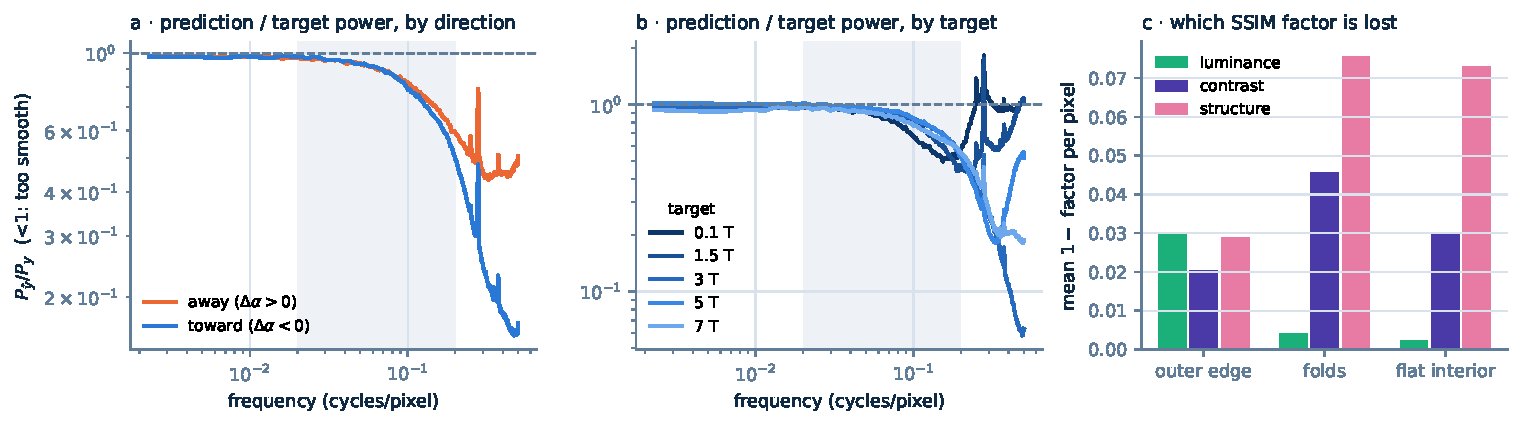
\includegraphics[width=\textwidth]{spectral/fig_error_smoothness.pdf}
\caption{Prediction power relative to the target, and the SSIM factor deficits by region.}
\label{fig:smooth}
\end{figure}

\begin{table}[H]
\centering\small
\begin{tabular}{llrrrrr}
\toprule
Panel & Group & $0.02$--$0.05$ & $0.05$--$0.1$ & $0.1$--$0.2$ & $0.2$--$0.3$ & $0.3$--$0.5$ \\
\midrule
\ref{fig:smooth}.a & all              & 0.958 & 0.893 & 0.715 & 0.447 & 0.299 \\
\ref{fig:smooth}.a & $\da>0$ (away)   & 0.955 & 0.896 & 0.743 & 0.546 & 0.453 \\
\ref{fig:smooth}.a & $\da<0$ (toward) & 0.961 & 0.891 & 0.697 & 0.401 & 0.200 \\
\ref{fig:smooth}.b & target 0.1\,T    & 0.947 & 0.843 & 0.592 & 0.866 & 0.974 \\
\ref{fig:smooth}.b & target 7\,T      & 0.940 & 0.866 & 0.693 & 0.461 & 0.218 \\
\bottomrule
\end{tabular}
\caption{$P_{\hat y}/P_y$ per band (cycles/pixel). Below 1: the prediction is smoother than
the target.}
\label{tab:smooth}
\end{table}

\begin{table}[H]
\centering\small
\begin{tabular}{llrrrrrr}
\toprule
Panel & Region & $1-l$ & $1-c$ & $1-s$ & $1-\mathrm{SSIM}$ & $\sigma^2_{\hat y}/\sigma^2_y$
      & smoother px \\
\midrule
\ref{fig:smooth}.c & outer edge    & 0.030 & 0.020 & 0.029 & 0.072 & 0.965 & 51\% \\
\ref{fig:smooth}.c & folds         & 0.004 & 0.046 & 0.076 & 0.115 & 0.791 & 77\% \\
\ref{fig:smooth}.c & flat interior & 0.002 & 0.030 & 0.073 & 0.101 & 0.856 & 69\% \\
\bottomrule
\end{tabular}
\caption{Mean per-pixel deficit of each SSIM factor ($l$ luminance, $c$ contrast, $s$
structure), all 168 transitions. Smoother px: share of windows with
$\sigma_{\hat y} < \sigma_y$.}
\label{tab:factors}
\end{table}

\begin{itemize}
  \item \textbf{The prediction is too smooth in every band, every group, both directions}
        (Table~\ref{tab:smooth}). Even away from high field it keeps only 74\% of the target's
        0.1--0.2 power. The one exception is target 0.1\,T above 0.2 cycles/pixel, where the
        target is noise floor and the prediction matches its power but not its phase
        ($P_e/P_y = 1.73$).
  \item \textbf{Structure is the largest loss} (0.073 in the flat interior, 0.076 on folds):
        the local pattern does not correlate with the target's. Luminance only matters at the
        outer edge (mask boundary).
  \item \textbf{Contrast is the second}, and it is a smoothness penalty: 77\% of fold windows
        and 69\% of flat windows have $\sigma_{\hat y} < \sigma_y$. Over whole slices the
        factors split the 0.0474 per-pixel deficit as luminance 0.0026, contrast 0.0149,
        structure 0.0322 (first order).
  \item Panel~\ref{fig:smooth}.b: the 0.29 cycles/pixel spike is in the prediction, strongest
        for target 0.1\,T.
\end{itemize}

\textbf{Verdict on the spectral-profile loss: dropped before implementation.}
\begin{itemize}
  \item The gate's premise was that away from high field, matching the target spectrum
        \emph{removes} detail. Measured: the prediction is already smoother than the target there
        too, so any spectrum-matching term (A1, A2 or A3) would \emph{add} power.
  \item Power added without correlation lowers SSIM: for fixed covariance, $c\cdot s =
        (2\sigma_{\hat y y} + C_2)/(\sigma^2_{\hat y} + \sigma^2_y + C_2)$ falls as
        $\sigma^2_{\hat y}$ grows. A log-spectrum loss has no way to ask for correlated power only.
\end{itemize}

\textbf{What the analysis points at instead: the contrast factor.}
\begin{itemize}
  \item Scale the prediction's local deviation by a gain $g$. Structure $s$ is
        scale-invariant, so it does not move; $c\cdot s = (2g\,\sigma_{\hat y y} + C_2)/
        (\sigma_y^2 + g^2\sigma_{\hat y}^2 + C_2)$, which for $C_2 \to 0$ peaks at
        $g = \sigma_y/\sigma_{\hat y}$, exactly where $c = 1$.
  \item So, unlike MSE, SSIM rewards restoring the local variance of detail the model
        \emph{already has}, without inventing new detail. Upper bound if $c = 1$ everywhere:
        about $+0.015$ local SSIM. A single global gain recovers only part of it, and $C_2$
        ($\sigma = 0.03$) shrinks the optimum in low-variance tissue.
  \item Consistent with two earlier results: checkpoint averaging + TTA (+0.0042) raised
        correlation and smoothed at the same time [\S40], and the rank-1 team's largest step
        was a GAN refinement (+0.024 SSIM), a sharpening stage [\S38.3].
\end{itemize}

% ======================================================================
\section{$\Delta\alpha$-gated spectral-profile loss: dropped}\label{sec:loss}

Dropped before implementation; reason in \S\ref{sec:analysis}, second pass. Kept for the
record, with the A0--A3 ablation it would have needed (never run):
\[
  \mathcal{L} = \mathcal{L}_{\text{current}}
  + \lambda\, g(\da_{s\to t}) \sum_{f \in [0.02,\,0.20]}
    \bigl|\log P_{\hat y}(f) - \log P_{y}(f)\bigr|,
  \qquad g \in \{1,\ \max(0,\da),\ \max(0,-\da)\}.
\]
\begin{itemize}
  \item Premise tested: away from high field the model leaves too much detail. Measured: it
        leaves too little, in every band and both directions (Table~\ref{tab:smooth}).
  \item Every arm would therefore add power, and a log-spectrum term cannot ask for
        \emph{correlated} power, which is the only kind SSIM rewards.
  \item Later trained anyway, to settle it by measurement rather than argument: negative
        (\S\ref{sec:losstest}).
\end{itemize}

% ======================================================================
\section{Recovering the contrast factor: E1 negative}\label{sec:next}

\textbf{E1, post-hoc detail gain (no training).} Script \texttt{scripts/detail\_gain\_sweep.py};
outputs \texttt{detail\_gain/} (\texttt{grid.csv}, \texttt{loso.csv}, \texttt{summary.csv},
\texttt{lpips.csv}).
\begin{itemize}
  \item Shipped predictions cached once through \texttt{predict\_slab} (shipped weights, TTA),
        scored with \texttt{eval\_holdout.score}'s SSIM / nRMSE (slab, source-zeroed).
  \item \emph{unsharp}: $\hat y + (g-1)(\hat y - G_\sigma * \hat y)$, $g \in \{1.1, 1.2, 1.3,
        1.5\}$, $\sigma \in \{1, 2\}$\,px, blur by normalised convolution inside the mask (a plain
        blur overshoots the brain boundary).
  \item \emph{window}: scale the deviation from the $7\times7$ local mean (the SSIM window) by
        $g \in \{1.05, 1.1, 1.2\}$, only where the prediction's local std exceeds
        $\tau \in \{0, 0.03, 0.06\}$. Closest to the derivation in \S\ref{sec:analysis}.
  \item Spot checks first: band-pass (difference of Gaussians) gains lost on all three
        transitions tried, so they were not swept.
\end{itemize}

\begin{table}[H]
\centering\small
\begin{tabular}{lrrrrr}
\toprule
Setting & $g$ & param & $\Delta$SSIM & $\Delta$nRMSE & improved \\
\midrule
window  & 1.05 & $\tau = 0.06$ & $-0.00005$ & $+0.00010$ & 24\% \\
window  & 1.05 & $\tau = 0.03$ & $-0.00006$ & $+0.00015$ & 26\% \\
unsharp & 1.1  & $\sigma = 1$  & $-0.00010$ & $+0.00015$ & 18\% \\
window  & 1.05 & $\tau = 0$    & $-0.00012$ & $+0.00021$ & 20\% \\
window  & 1.1  & $\tau = 0.06$ & $-0.00020$ & $+0.00031$ & 9\% \\
unsharp & 1.5  & $\sigma = 2$  & $-0.00550$ & $+0.00671$ & 0\% \\
\bottomrule
\end{tabular}
\caption{In-sample, 168 ranked transitions, against the shipped prediction (local SSIM 0.95113).
Best five of 17 settings plus the strongest; all 17 in \texttt{detail\_gain/grid.csv}.
Improved: share of transitions where the setting beats the shipped prediction.}
\label{tab:e1}
\end{table}

\begin{table}[H]
\centering\small
\begin{tabular}{lrrr}
\toprule
Rule & Held-out $\Delta$SSIM & $\Delta$nRMSE & improved \\
\midrule
one global setting                 & $0$         & $0$          & 0\% \\
one setting per target field       & $-0.00001$  & $+0.00002$   & 3\% \\
best setting per transition, oracle & $+0.00004$ & $+0.00001$   & 32\% \\
\bottomrule
\end{tabular}
\caption{Leave-one-subject-out: fit on two subjects, score on the third, all three rotations.
The global rule picks the identity in every fold; per target, only 7\,T picks a gain (window,
1.05) in two folds, and it loses on the held-out subject. The oracle is in-sample by
construction.}
\label{tab:e1loso}
\end{table}

\begin{itemize}
  \item \textbf{No sharpening setting raises SSIM}, globally, per target field, or in
        leave-one-subject-out. Even the per-transition oracle is worth $+0.00004$, a
        twenty-fifth of the $0.001$ ruler [\S32].
  \item Why the derivation in \S\ref{sec:analysis} did not transfer: the optimum
        $g = \sigma_y/\sigma_{\hat y}$ assumes $C_2 \to 0$. 27--50\% of brain windows have
        target $\sigma_y < 0.03 = \sqrt{C_2}$ (spot checks, one slice per transition); there
        $C_2$ dominates and a gain helps only if the target's deviation regresses on the
        prediction's with slope above 1, which is the MSE criterion a posterior-mean prediction
        already satisfies. Where $\sigma$ is large, the per-window optimum $\sigma_y/\sigma_{\hat y}$
        varies too much for one gain (31\% of flat windows are already rougher than the target).
  \item So the contrast deficit is target variance the prediction cannot correlate with, not
        shrinkage of detail it has. Recovering it needs information, the same as the
        structure deficit; post-processing cannot.
  \item Side result, the first slab-scored local number for the shipped model on the fixed
        harness [\S41]: \textbf{local 0.95069} (180 transitions), nRMSE 0.08869, LPIPS 0.07044,
        against challenge 0.913652. Scored through \texttt{predict\_slab}, not
        \texttt{eval\_holdout.predict}.
\end{itemize}

\textbf{E2, SSIM loss weight above 0.5: not run.}
\begin{itemize}
  \item Its rationale was ``the trained version of E1'': pull the output toward variance
        matching. E1 shows the variance the prediction lacks is not recoverable by scaling, so
        that rationale is gone.
  \item A higher weight could still change \emph{which} detail the network produces, but there
        is no measurement here that predicts it, and \S28.6 found the weight response
        non-monotone with $\pm0.003$ epoch-to-epoch swings. Not worth a fine-tune on this
        evidence.
\end{itemize}

% ======================================================================
\section{Spectral-profile loss, trained: negative}\label{sec:losstest}

Why run what \S\ref{sec:loss} dropped: E1 only shows the shipped prediction cannot be
sharpened \emph{after the fact}. A trained term could still add detail the network can infer
from its input, and on $\da > 0$ transitions (target smoother than source) that detail is in
the input. One fine-tune settles it.

\textbf{Setup.} Config \texttt{task3\_mc\_ssim\_slice\_spec.toml}; term in
\texttt{components/training/task3.py} (\texttt{spectral\_weight}, \texttt{spectral\_gate},
\texttt{spectral\_alphas}; weight 0 skips it).
\[
  \mathcal{L} = \mathcal{L}_{\text{shipped}}
  + \lambda\, \frac{1}{B}\sum_{b} \max(0, \da_b)\; \frac{1}{18}\sum_{r=1}^{18}
    \bigl|\log P_{\hat y_b}(r) - \log P_{y_b}(r)\bigr|,
  \qquad \lambda = 0.025,
\]
with $P(r)$ the \texttt{rfft2} power of the $368\times448$ training crop summed over ring $r$ of
width 0.01 cycles/pixel in $[0.02, 0.20]$, float32 outside autocast.
\begin{itemize}
  \item \textbf{Arm A2 only}, $g = \max(0,\da)$. A1 ($g = 1$) and A3 ($g = \max(0,-\da)$) charge
        transitions where the detail is not in the input; if A2 loses, they have less reason to
        win.
  \item \textbf{$\lambda$}: at step 0 on the start checkpoint the gated term averages 0.164
        against a base loss of 0.0405 (12 batches; batch 0 reproduces the logged step-0 loss
        0.042617), so $\lambda = 0.025$ makes it 10\% of the total. A $\lambda$ sweep would
        cost three fine-tunes.
  \item Same seed, start checkpoint (\texttt{widened4\_from\_e25.pt}) and 8 epochs as the
        shipped run, which is the control. Mean of e6/e7/e8, 4-flip TTA, scored with
        \texttt{scripts/spectral\_loss\_eval.py} on the path of the shipped local 0.95069
        (verified to reproduce it to $10^{-16}$). Outputs in \texttt{spectral\_loss/}.
\end{itemize}

\begin{table}[H]
\centering\small
\begin{tabular}{lrrrrrrrr}
\toprule
Epoch & 1 & 2 & 3 & 4 & 5 & 6 & 7 & 8 \\
\midrule
$1-\mathrm{SSIM}$, control  & 0.04411 & 0.04182 & 0.04081 & 0.03990 & 0.03919 & 0.03865 & 0.03808 & 0.03748 \\
$1-\mathrm{SSIM}$, spectral & 0.04487 & 0.04276 & 0.04171 & 0.04095 & 0.04025 & 0.03968 & 0.03915 & 0.03865 \\
gap                         & 0.00076 & 0.00094 & 0.00089 & 0.00106 & 0.00106 & 0.00103 & 0.00107 & 0.00117 \\
spectral term               & 0.0443  & 0.0363  & 0.0340  & 0.0324  & 0.0309  & 0.0300  & 0.0297  & 0.0288  \\
\bottomrule
\end{tabular}
\caption{Training-loss epoch means. The gated term falls from 0.164 at step 0 to 0.029, so the
network did learn it; the SSIM gap to the control opens in epoch 1 and never closes.}
\label{tab:spectrain}
\end{table}

\begin{table}[H]
\centering\small
\begin{tabular}{lrrrrrr}
\toprule
Group & $n$ & SSIM & $\Delta$SSIM & $\Delta$nRMSE & $\Delta$LPIPS & improved \\
\midrule
ranked              & 168 & 0.94995 & $-0.00118$ & $+0.00208$ & $+0.00034$ & 4 \\
gate on ($\da>0$)   & 81  & 0.95065 & $-0.00149$ & $+0.00216$ & $-0.00077$ & 2 \\
gate off ($\da<0$)  & 87  & 0.94929 & $-0.00089$ & $+0.00200$ & $+0.00138$ & 2 \\
target 0.1\,T       & 36  & 0.94008 & $-0.00232$ & $+0.00206$ & $+0.00044$ & 0 \\
target 7\,T         & 36  & 0.96287 & $-0.00080$ & $+0.00295$ & $-0.00044$ & 4 \\
\bottomrule
\end{tabular}
\caption{Local, paired per transition against the shipped model (ranked 0.95113). Improved:
transitions where SSIM rose; all four are 7\,T targets. Per modality: T1W $-0.00081$, T2W
$-0.00121$, T2FLAIR $-0.00153$.}
\label{tab:specscore}
\end{table}

\begin{figure}[H]
\centering
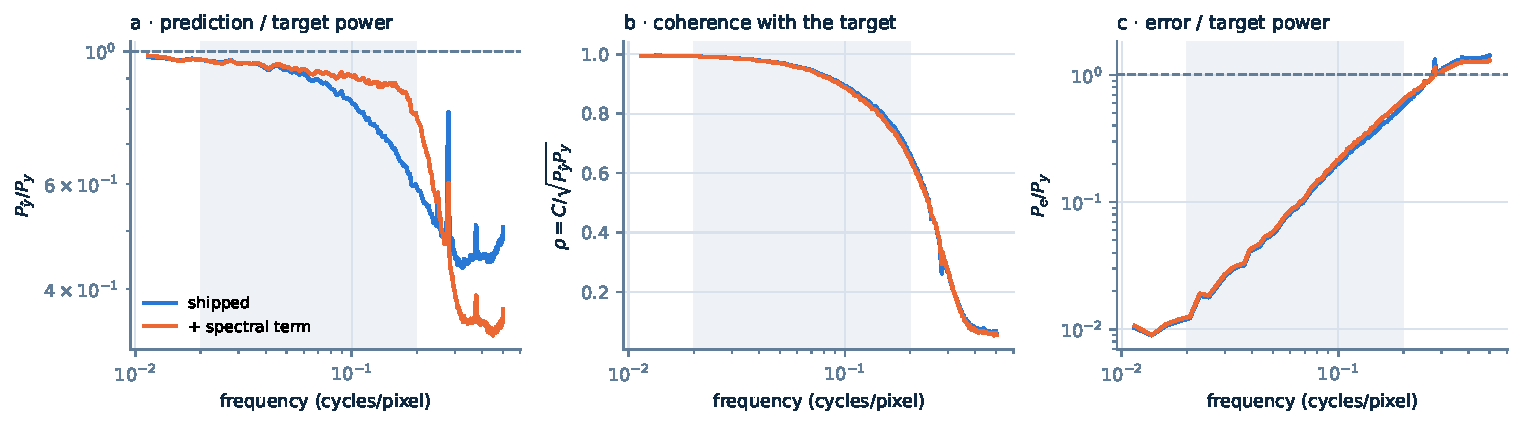
\includegraphics[width=\textwidth]{spectral/fig_spectral_loss.pdf}
\caption{Gate-on transitions (81 ranked), shipped against the spectral-loss model. Shaded: the
band the term acts on. $C = (P_{\hat y} + P_y - P_e)/2$ is the cross power, exact because
$e = \hat y - y$ is transformed on the same padded grid.}
\label{fig:specloss}
\end{figure}

\begin{table}[H]
\centering\small
\begin{tabular}{llrrr}
\toprule
Panel & Group, band (cycles/px) & $P_{\hat y}/P_y$ & coherence $\rho$ & $P_e/P_y$ \\
\midrule
\ref{fig:specloss} & gate on, 0.02--0.05 & 0.955 $\to$ 0.956 & 0.987 $\to$ 0.986 & 0.027 $\to$ 0.028 \\
\ref{fig:specloss} & gate on, 0.05--0.10 & 0.896 $\to$ 0.925 & 0.948 $\to$ 0.945 & 0.102 $\to$ 0.107 \\
\ref{fig:specloss} & gate on, 0.10--0.20 & 0.743 $\to$ 0.882 & 0.833 $\to$ 0.822 & 0.307 $\to$ 0.339 \\
\ref{fig:specloss} & gate on, 0.20--0.30 & 0.546 $\to$ 0.633 & 0.535 $\to$ 0.533 & 0.756 $\to$ 0.785 \\
                   & target 0.1\,T, 0.10--0.20 & 0.592 $\to$ 1.000 & 0.643 $\to$ 0.639 & 0.603 $\to$ 0.722 \\
                   & gate off, 0.10--0.20 & 0.697 $\to$ 0.670 & 0.818 $\to$ 0.815 & 0.332 $\to$ 0.336 \\
\bottomrule
\end{tabular}
\caption{Shipped $\to$ spectral-loss model, ring energies summed over the group's ranked
transitions (\texttt{error\_spectrum\_analysis.py} run on both). Full table in
\texttt{spectral\_loss/bands.csv}.}
\label{tab:specbands}
\end{table}

\begin{itemize}
  \item \textbf{The term did what it asks.} On gated transitions the prediction's 0.1--0.2 power
        rose from 0.743 to 0.882 of the target's; on 0.1\,T targets, where the gate is largest
        ($\da$ 0.85 to 1.72), it reached 1.000.
  \item \textbf{None of the added power is coherent with the target.} Coherence is flat or
        down in every band (0.833 $\to$ 0.822 at 0.1--0.2), so error power rose with the
        prediction's (0.307 $\to$ 0.339; 0.1\,T targets 0.603 $\to$ 0.722). The network met the
        term by turning up the gain on detail it already had, the trained form of E1, which
        \S\ref{sec:next} already showed lowers SSIM.
  \item \textbf{SSIM falls most where the term acts}: gate on $-0.00149$, target 0.1\,T
        $-0.00232$. 164 of 168 transitions are worse, so this is not the noise of the $0.001$
        ruler [\S32], though it is in-sample (all three subjects are trained on).
  \item \textbf{It also spills over.} Ungated transitions got smoother (0.697 $\to$ 0.670) and
        lost $-0.00089$; the term shares every weight with them.
  \item LPIPS improves only where the term acts ($-0.00077$, gate on): the LPIPS-for-SSIM trade
        of \S28.1 and \S40 once more.
  \item \textbf{Closed.} Together with E1 this answers the question for any spectrum- or
        variance-matching objective on this model: the missing power is not coherent with
        anything in the input that the network can reach. Remaining SSIM needs information, not
        a different loss shape.
  \item Challenge: zip built (\texttt{submissions/task3\_mc\_ssim\_slice\_spec\_avg\_tta}),
        \pending[not submitted].
\end{itemize}

% ======================================================================
\section{Change log}\label{sec:log}

\begin{itemize}
  \item 2026-10-07: report started; \S\ref{sec:start}--\S\ref{sec:plan} written.
  \item 2026-10-07: \texttt{scripts/error\_spectrum\_analysis.py} run on 180 transitions;
        results and gate verdict in \S\ref{sec:analysis}.
  \item 2026-10-07: second pass (prediction spectrum, SSIM factor split). Prediction too smooth
        everywhere; spectral-profile loss dropped; contrast-factor plan in \S\ref{sec:next}.
  \item 2026-10-07: E1 (post-hoc detail gain, 17 settings, leave-one-subject-out) negative; E2
        not run; report closed.
  \item 2026-10-07: reopened. Spectral loss (arm A2) trained after all
        (\S\ref{sec:losstest}): power up, coherence flat, local SSIM $-0.00118$.
\end{itemize}

\end{document}
